\section{Example: Interface to {UNDUMAG}} \label{ex11}

UNDUMAG \cite{undu} is a code develloped at HZB/BESSY to calculate the
magnetic fields of undulators and other magnetic structures.

WAVE has an interface to \U to calculate the field of an APPLE II
undulator and a planar hybrid undulator with iron poles. The parameters of the undulator and
magnets are given in the namelist \scap{\$UNDUMAG}.

The files

\cboxs{undumag.exe}

and

\cboxs{undumag\_nam.tmp}

must be installed in

\cboxs{\$WAVE/undumag}

These file names are defined by \scap{CHUNDUMAG} and \scap{CHUNDUNAM}
in \scap{\$UNDUMAG}.

To try this example, enter:

\cbox{\senv \grau \\
python3 ../python/wave\_example\_11.py\\
cp \$WAVE/input/wave\_example\_11.in wave.in\\
wave
}\\

\U writes some output files. Have a look to
\gtis{undumag.log} and
\gtis{undumag.beff}. There is also some graphical output, see
\gtis{undumag*.eps}.

The geometry of the undulator magnet structure is
shown in \gtis{undumag.eps}.

\begin{figure}[ht]
    \centering
    \framebox(12.5,8){
      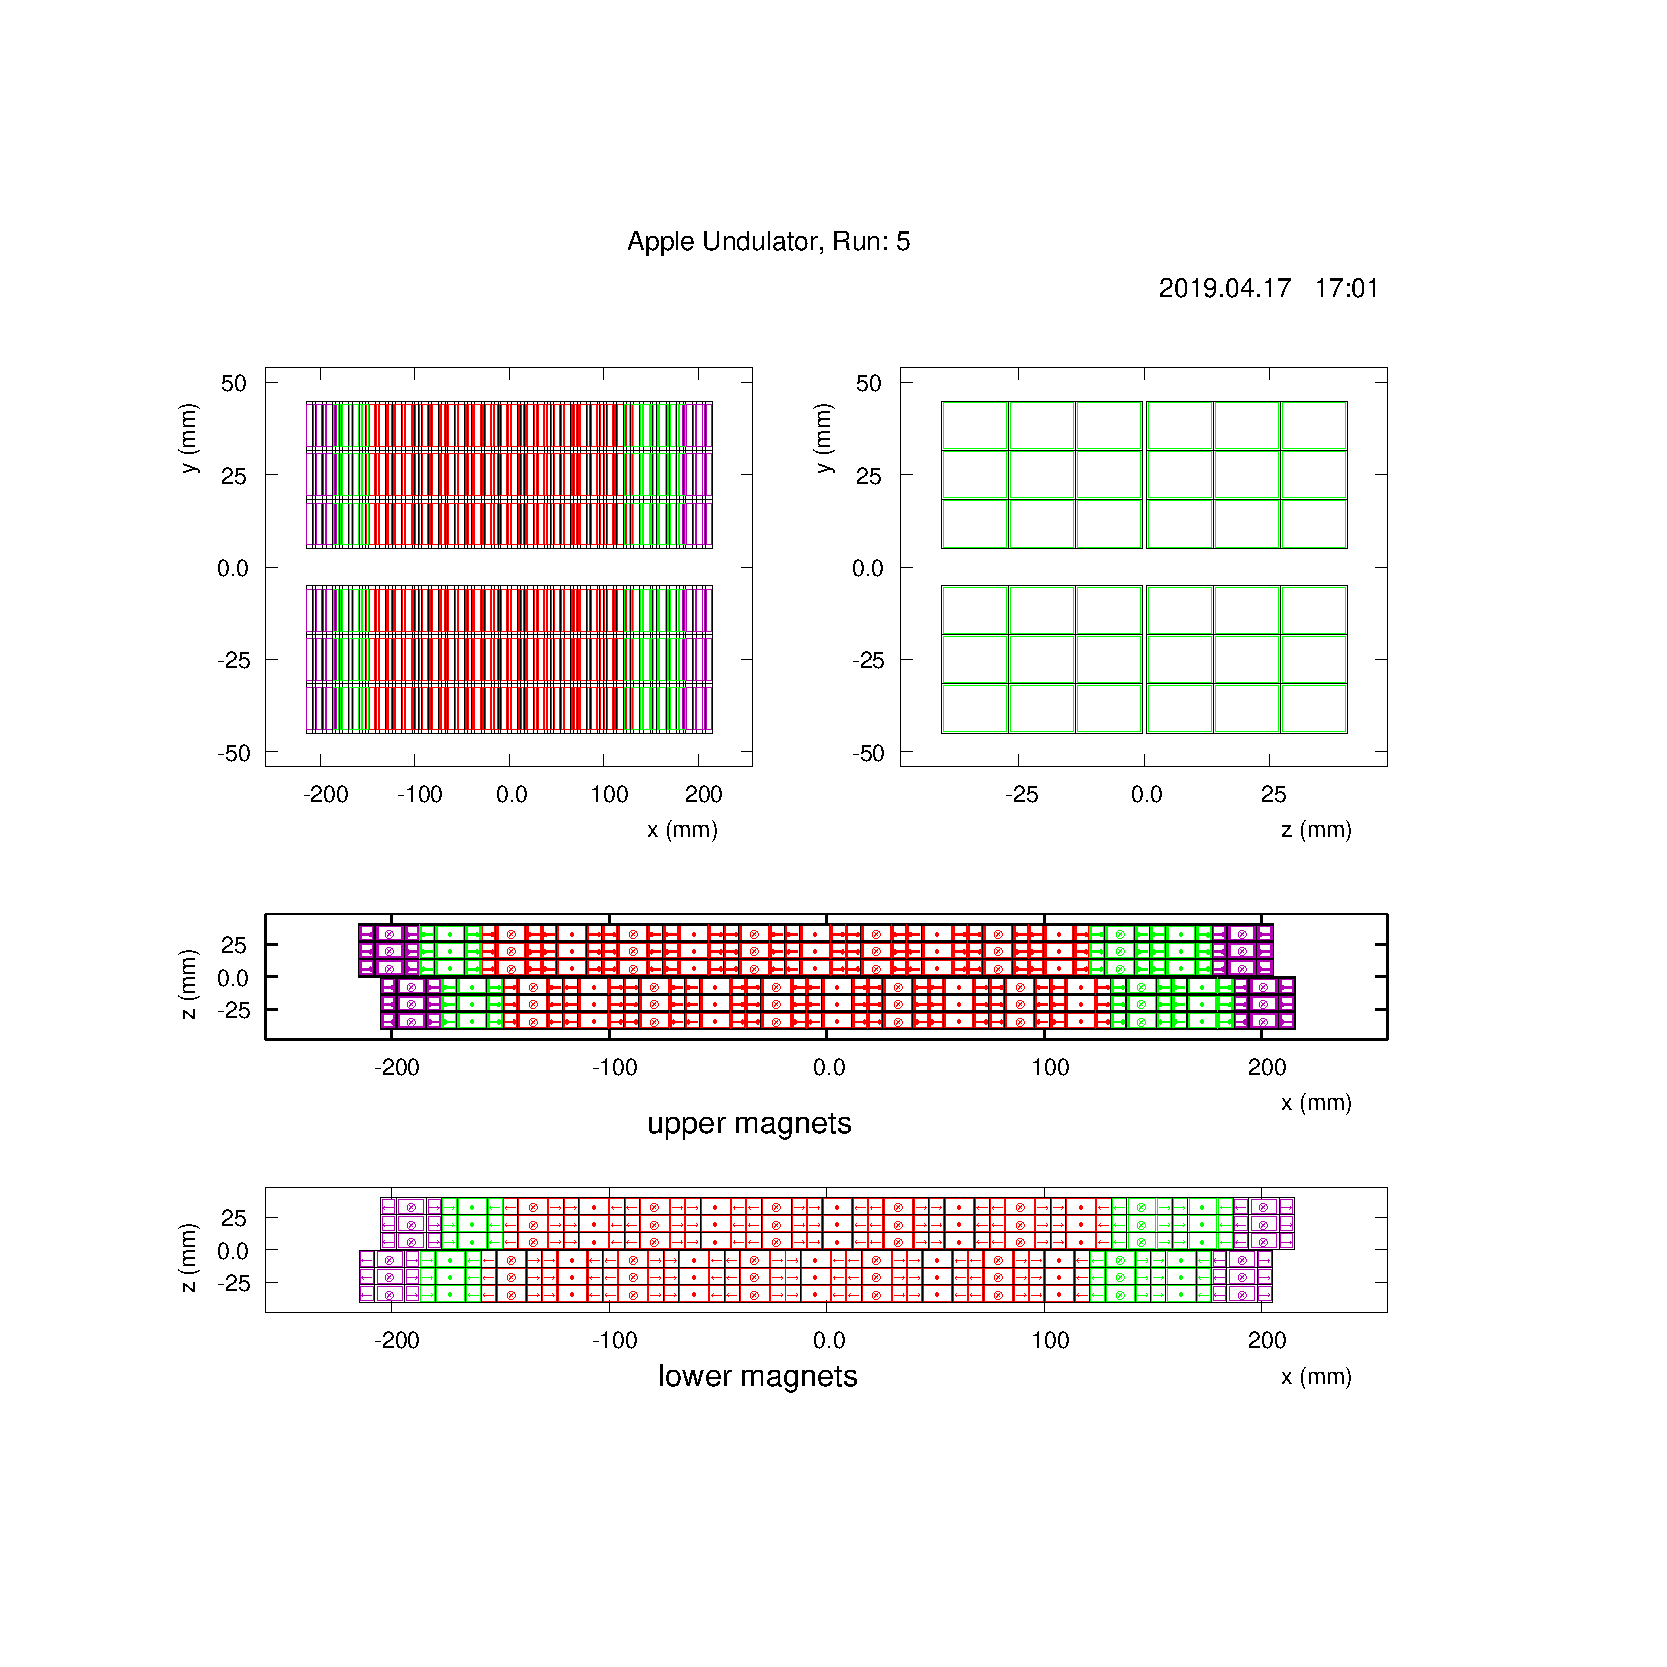
\includegraphics[width=0.65\textwidth]
      {pics/wave_example_11_1.pdf}
    }
    \caption{Example of an APPLE-II undulator}
    \label{ex11fig1}
\end{figure}

The figure \ref{ex11fig1} shows the magnetic structure and also the
segementation of the magnets. Be aware, that \U can be very memory consuming. Therefore, you
must limit the number of periods and the segmentation of the magnets.
These parameters can be set in the namelist \scap{\$UNDUMAG} or by
using \WSHE.

The namelist \scap{\$CONTRL} holds the parameter \scap{KBUNDUMAG},
which triggers for

\cboxs{ KBUNDUMAG=2}

the \U run.

If you want to use the ouput
of \U instead for a subsequent \W run, just set

\cboxs{KBUNDUMAG=1}

In this case, the file \gtis{undumag.wav} is used by \W. This is
espacially useful, if the \U run is time consuming. The file
\gtis{undumag.wav} contains all voxels of the magnetic setup and
their magnetization as calculated by \U.
WAVE calculates then the contribution of each
voxel applying the current sheet method. This can also be rather time
consuming. Therefore, it might be better to calculate a field map
first, with \U or WAVE for later use.

In special cases, it might be helpful to edit \gtis{undumag.nam} and
\gtis{undumag.clc} and not letting \W set up them form the templates.
This can be achieved by setting \scap{KBUNDUMAG=-1}. This is equivilent to
run \U seperately and then setting \scap{KBUNDUMAG=1}, which
also can be achieved by the command:

\cbox{undumag}

The namelist \scap{UNDUMAGN} contains the parameters to change the
gap, shift of the undulator and other parameters to control
\U, e.g. the definition of the field map to be calculated.
Of course, a field map can also be written by \W, check the variable
\scap{IWBMAP} in \wie.

The advantage of using \U over the REC-undulators of
exampel \scap{4} is the realistic simulation of the interaction of the
magnets. One effect e.g., which can not be simulated with the model of
example \scap{4} is the effect on the endmagnets and hence on the first and
second field integrals when the shift is changed. For more details and
options refer to the namelist \scap{\$UNDUMAGN} in  {\it wave.in}.\\[0.5cm]

{\bf Periodic Field expansion\\[0.5cm]
}
If the segmentation of the items in \U is fine, the number of voxels
becomes very large and slows down the computation significantly. On
the other hand, the periodic field is a genuine characteristic of
undulators. Therefor, \W offers a method to repeat a part of the
field periodically.

Please check the namelist
\scap{\$B0SCGLOBN} in \wie. This namelist offers options of global modification
of the magnetic field configuration, e.g. shifting or scaling the field.

We use this namelist to expand the undulator by twenty periods and
set:\\

\cboxs{KBUNDUMAG=1\\
XSHIFT=0.56\\
IPERIODG=-1\\
XPERWMN=0.0\\
XPERWMX=1.12\\
PERIODG=0.056\\
PEROFFG=0.028
}\\

The variable \scap{IPERIODG=-1} selects the mode the periodic part of the
field is treated.

\scap{XPERWMN=0.0} and \scap{XPERWMX=1.12} define the region
of the periodic part, while \scap{PERIODG=0.056} and \scap{PEROFFG=0.028} define
the period to be repeated.

Since these setting would shift the center
of the device, we correct this with \scap{XSHIFT=0.56} to keep the center
of the undulator at the origin.

We save \wi with these settings and run \W. The result is the field
in Fig.~(\ref{ex11fig2}).

\begin{figure}[ht]
    \centering
%    \framebox(12.5,8){
      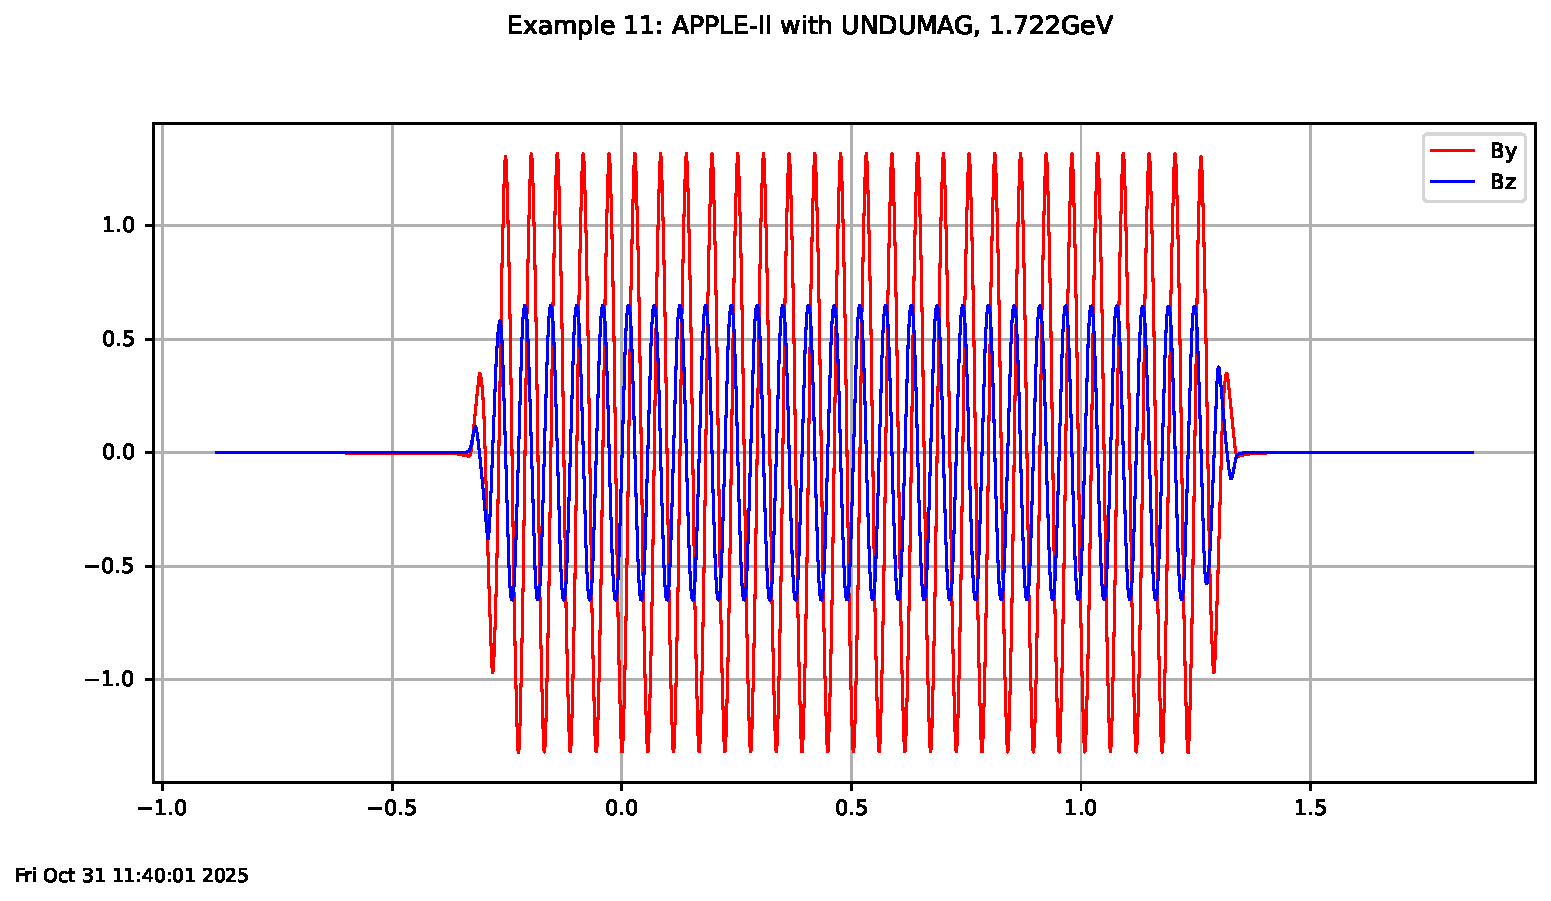
\includegraphics[width=0.65\textwidth]
      {pics/wave_example_11_fig1.pdf}
%    }
    \caption{Field of the expanded undulator}
    \label{ex11fig2}
\end{figure}

